\section{Research Plan}

Figure \ref{fig:flow} shows the basic outline of a proposed workflow
and components needed to support feedback-driven mutation testing.
These components serve to organize the research plan.

\subsection{Mutant Generator}
\label{sec:anylangplan}

The most widely-used mutation testing tool in the real world
is PIT~\cite{pittest}, which targets Java bytecode.  There are recent attempts
to provide the same kind of support for other languages, especially C, by
targeting LLVM IR~\cite{HaririLLVM,Mart}.  This poses several problems for
feedback-driven mutation testing.
First, bytecode- or IR-level mutation works well to compute a
score for a test suite, but is not not suitable for presentation to developers
or test engineers, who need to reason about a mutant's implications for their
source or test code.   Java developers
think in terms of Java, not compiled bytecode; C and C+++ developers certainly
do not generally understand LLVM IR.  Even when possible, translation may not help: a bytecode-level
mutation may not have a simple source-level equivalent, especially if the
bytecode has been optimized.  Second, features that help identify semantically
similar (or dissimilar) mutants are hard to identify at the bytecode level.  Even if the mutant
is, for example, a constant replacement in one case and an arithmetic operator
replacement in another, the fact that both take place inside an argument to a
logging function with an {\tt INFO} argument may be enough to predict that their
effects are redundant.
Finally, IR-specific tools are by construction limited to their associated
language ecosystems, excluding a large body of code written in other languages,
as well as project-specific DSLs.
Moreover, the vast majority of software projects are written
in multiple languages~\cite{Ray2014}.  Our desire for real-world applicability
thus motivates polyglot analysis and testing infrastructure.

Thus, our first research task is to develop a novel {\tt mutant generator} that
(1) operates at the source level, with output that is easy for developers to
understand and the framework to analyze; (2) is, as much as possible,
\emph{language independent}, and applicable to projects written in a
heterogeneity of languages; and finally (3) is efficient.  The PIs' recent
advances in universal mutation~\cite{regexpMut,universalmutator} and
language-agnostic declarative program transformation using parser
combinators~\cite{rvt-ppc} provide key motivation and starting points for this
component.

\subsubsection{Background and preliminary work}

% CLG: I'm tempted to cut some of the universal mutator content.  I view it as
% important in that it shows that language-agnostic, syntax-driven mutation is
% viable for mutation testing, but since we're mostly building on Comby here, we
% need the space for that

%\begin{figure}
%{\scriptsize
%\begin{tabularx}{0.75\textwidth}{XXX}
%\verb|\+ ==> -| & \verb|== ==> !=| & \verb|(\D)(\d+)(\D) ==> \1(\2+1)\3|\\
%\verb|\+ ==> *| & \verb|== ==> <| & \verb|(\D)(\d+)(\D) ==> \1(\2-1)\3|\\
%\verb|\+ ==> /| & \verb|== ==> >| & \verb|(\D)(\d+)(\D) ==> \g<1>0\3|\\
%\verb|".+" ==> ""| & \verb|while ==> if| & \verb|(^\s*)(\S+.*)\n ==> \1\2\n\1break;\n|\\
%{\tt \\+ ==> *} & {\tt != ==> <=} & {\tt (\D)(\\d+)(\D) ==> \\1\\2-1\\3}\\
%{\tt \\+ ==> /} & {\tt != ==> >=} & {\tt ".+" ==> ""}\\
%{\tt \\+ ==> \%} & {\tt != ==> >=} & {\tt (^\\s*)(\\S+.*)\\n ==> \\1\\2\\n\\1break;\\n}\\
%\end{tabularx}
%}
%\caption{Some universal mutation rules}
%\label{fig:rules}
%\end{figure}

%The PI's combined prior work provides evidence for the feasibility of any-language mutation:

\paragraph{The universalmutator.} First, PI Groce and colleagues
released a fully functional, regular-expression-based mutant
generator~\cite{regexpMut,universalmutator}.
The {\tt universalmutator}
does not attempt to parse source code, but simply defines mutation
operators by a set of regular-expression-defined text transformations.  These
are organized into a hierarchy, so that if a program is, e.g., written in Swift,
the ``universal'' mutation operators that apply to all programming languages are
first applied, then operators for ``C-like'' languages, and finally a set of
Swift-specific rules are applied.  %Figure \ref{fig:rules} shows some of the
%``universal'' rules applied to all languages.

Importantly,  PI Groce demonstrated that the {\tt universalmutator} tool generated
numbers of mutants and kill ratios for Java code comparable to
PIT~\cite{pittest} and Major~\cite{Major}.  For falsification-driven
verification, the regular-expression-based approach produced mutants of equal
value to those produced by Andrews' tool~\cite{mutant} and Muupi~\cite{muupi}
for C and Python, respectively.
This demonstrates that multi-language, syntax-driven, source-level mutation is
\emph{feasible} and, indeed, effective, producing results competitive with
state-of-the-art single-language mutation tools.  It is already being
used, for instance as the Ethereum foundation recommended tool for mutation testing of
Solidity smart contracts.
However, it has significant limitations for long-term utility,
motivating this project: Because the source
code is not parsed, and applies regular expressions to lines of code, not
larger blocks, the technique generates many mutants that are invalid
and cannot be compiled, or that are trivially equivalent because they, e.g.,
mutate ``source code'' in a large comment block.
%Integrating mutation
%generation with execution is currently supported, but extending it to new
%languages or build systems is hard for users, requiring writing considerable
%Python code or complex shell scripts.
%It is currently impossible to define
%mutation operators that apply to blocks of code rather than text within a single
%line, and standard regular expressions are not really suited to describing code
%constructs such as blocks, functions, classes, or structs.  Natural formatting
%of, e.g., an s-expression in a LISP-family language can hide opportunities for
%mutation, such as switching argument orders.
Fundamentally, regular expressions are
only occasionally a natural notation for expressing source-level mutation;
source in all languages differs from arbitrary unstructured strings.

\paragraph{Comby: Declarative, any-language transformation.} Fortunately, recent work by PI
Le Goues and collaborators introduced a powerful new representation to
declaratively transform richer syntactic structures in programs across multiple
languages~\cite{rvt-ppc}. The key innovation is to convert declarative
transformation templates into parsers that directly match and transform source
code of interest. Parser
combinators~\cite{Hutton96monadicparser} define how to match nested structures (much like traditional AST
visitor traversals) but without the need to define or build an intermediate AST.
% intermediate step of building the AST.
% or AST, but I'm going with parse tree because it's specific to syntax.
Our parser combinator mechanism elegantly encapsulates the complexity of
heterogeneous, multi-language syntax as a composition of small parsers (some
being language-specific, and others being language-general). Conversely, defining and
building a generic parse tree data structure (i.e., to encompass the complexity
of multi-language syntax, which may be inherently incompatible across languages)
\emph{after} parsing is comparably difficult.

This work has already shown its practical utility by performing lightweight
refactors in more than 10 languages (including those targeted by {\tt
  universalmutator}). The associated tool, {\tt comby}~\cite{comby-github},
enables a new language-general way of expressing transformations that regular
expressions cannot typically recognize (e.g., nested code blocks). We showed
that {\tt comby} has equivalent expressive power for a variety of nontrivial syntactic
transformations in existing language-specific refactoring tools. {\tt Comby} is
highly performant at scale (owing to the parser-driven approach), processing
upwards of a quarter billion lines of code in 42 minutes (parallelized over 20 cores).

%Current mutation testing approaches largely rely on either
%sophisticated language-specific tools that fail to generalize to other
%languages~\cite{Major} or rudimentary textual manipulation~\cite{mutant} that is
%fundamentally limited in effectiveness.
Coupling with declarative syntax manipulation that goes beyond the limits
of regular expressions  promises to yield more effective mutation testing by (a) targeting more
sophisticated properties of programs, and (b) delivering more user-accessible
tools for developing mutation transformations. Our joint advances in
real-world tooling (i.e., in {\tt universalmutator} and {\tt comby}) suggest that
this goal is imminently feasible.  At heart, this line of work
represents the conviction of the PIs that mutation testing (like
automated program repair) is simply
an instance of the general field of automated program
transformation~\cite{Ptransform}.

We have jointly used ideas from universalmutator and comby to develop
a novel approach to compiler fuzzing, supported by a tool~\cite{aflcompfuzz} (with
industrial users and 47 stars on GitHub), which has resulted in
discovery of more than 80 bugs in production compilers, and a
substantial bug bounty from the Ethereum foundation.  Work from this
project will benefit that effort, and we expect work from that effort
to benefit polyglot mutation.

\subsubsection{Proposed work: Any language mutation}
\label{subsubsection:any-language}

Our goal is a source-level mutant generator that can apply to any language,
maximizing applicability and usability.
 The {\tt
  universalmutator} provides an initial source of mutants that
satisfies this requirement for initial experimentation, but for
long-term effectiveness is both inefficient and inexpressive.


% The source of all mutants to be presented to the user is the mutant
% generator, and in order to maximize the effectiveness of the approach,
% this proposal aims to allow effective generation of mutants for any
% programming
% language or DSL, with minimal additional effort. The
% current implementation avoids parsing to such an extent that it
% generates numerous useless mutants embedded in code comments, or that
% are obviously syntactically invalid.  While avoiding a parser-based
% approach, simple additional constraints could avoid this, without
% adding burden on users, such as allowing the definition of a
% language's comment mechanisms, and not producing mutants inside
% comments.  More generally, a mechanism for disabling mutation in
% contexts defined in the same way as mutation operators would handle
% other, even project-specific, constraints (e.g., never mutate inline
% assembly in C/C++).  A problem with the current representation of
% mutation operators and such contexts is that regular expressions are
% currently applied only at the line level, and in any case are not
% effective for defining such fundamentally non-regular aspects of code
% as blocks and nested delimiters.  A key goal in this project is to greatly
% enhance
% % the regular-expression language (without losing its simplicity
% %for ``normal'' operators) with the ability to express, in a
% %language-independent, syntactic form, such context-dependent aspects
% %of code.
% the expressity of transformations (e.g., operators for multi-line, context-dependent program fragments) while retaining the simplicity of specifying usual % or "normal" operators as above, but I'm not sure what normal is? Is Fig. 1 representative?
% operators.

We therefore propose to use {\tt comby}~\cite{comby-github, rvt-ppc} for specifying
transformations and generating mutants. {\tt Comby} uses
declarative templates that describe before/after changes for program fragments. For example, the following transformation swaps the first two arguments of the function {\tt memcpy}:

\begin{figure}[!h]
\centering
\begin{BVerbatim}[commandchars=\\\{\}]
memcpy(\textcolor{blue}{:[1]}, \textcolor{ForestGreen}{:[2]}, :[3]) ==> memcpy(\textcolor{ForestGreen}{:[2]}, \textcolor{blue}{:[1]}, :[3])
\end{BVerbatim}
\end{figure}

Hole syntax \verb|:[1]| binds syntax to a variable. A unique property of {\tt
  comby} templates is that variables
\emph{only} bind to syntax that occurs
inside well-balanced delimiters (like parentheses), whitespace is handled intelligently, %(i.e., a space indicates any whitespace, including newlines)
and syntax otherwise matches literally. % (i.e., with minimal metasyntax).
Concretely, this means that the template above seamlessly transforms syntax structure in complex fragments as in the following:

\begin{figure}[!h]
\footnotesize
\begin{subfigure}[t]{.47\textwidth}
\centering
\begin{Verbatim}[commandchars=\\\{\}]
memcpy(\textcolor{blue}{*stream->main_data + stream->md_len},
       \textcolor{ForestGreen}{mad_bit_nextbyte(&stream->ptr)},
       frame_used = md_len - si.main_data_begin);
\end{Verbatim}
\end{subfigure}%
\begin{subfigure}[t]{.04\textwidth}
\begin{verbatim}

==>

\end{verbatim}
\end{subfigure}%
\begin{subfigure}[t]{.47\textwidth}
\begin{Verbatim}[commandchars=\\\{\}]
memcpy(\textcolor{ForestGreen}{mad_bit_nextbyte(&stream->ptr)},
       \textcolor{blue}{*stream->foo_data + stream->md_len},
       frame_used = md_len - si.foo_data_begin);
\end{Verbatim}
\end{subfigure}
\normalsize
\end{figure}
% The above fragment comes from real example: https://sourcegraph.com/github.com/markjeee/libmad/-/blob/layer3.c#L2637
% The above example of in a live example here: bit.ly/2Nmh3v2

At a high-level, {\tt comby} performs
% actual
context-free
parsing of syntactic structures that typically correspond to nested
expressions and blocks in the underlying AST; regular expressions are not powerful enough to recognize such program terms in general. Templates offer a \emph{declarative} description for matching and rewriting these structures in a way that is syntactically close to the source code.
In addition, {\tt comby} can distinguish between code, strings, and comments. Templates contextually match these dimensions of a program. % (which are common to virtually all languages)
% Compared to regular-expressions, {\tt comby} can match on nested structures, can discriminate between code, data (strings), and comments on a language-aware basis.
{\tt Comby} is language-aware in the sense that small language
definitions describe whether syntax should be balanced (e.g.,
parentheses or braces) or delineate strings or comments. These
definitions describe a coarse structural decomposition of programs (as
typically understood by compilers) rather than just a sequence of
characters (as treated by regex). Language definitions already exist
for 20+ languages, and {\tt comby} supports a simple extension
mechanism for new languages (e.g., Solidity) or custom DSLs (\url{https://comby.dev/\#faq-language-support}).
One ongoing limitation of mutation testing is that tools are often research
projects, and eventually become unusable due to lack of support, even in
mainstream languages such as Java and C~\cite{MutChoice}.
This is because mutation tools that fully parse a language and guarantee generation of
valid programs in the source language are complex, hard-to-maintain-and-extend
systems; language complexity makes such a tool for C++, for example, an extremely daunting task. From this development and maintenance perspective, {\tt comby} provides a considerable benefit in being able to adapt to new language syntax and tree structures at a coarse level, while maintaining a crucial language-aware ability for recognizing and parsing high-level program constructs.

Accessible structural syntax manipulation can achieve a leap in
expressivity and effectiveness for mutation testing. % a cite to substantiate "based on what" would be nice
For one, targeted structural and contextual changes are
more likely to produce well-formed syntactic programs
that exercise interesting paths in a test suite.
We propose to extend {\tt universalmutator}
to generate mutants from {\tt comby} templates, and to evaluate the efficacy of
multi-language mutation testing with structural code changes.  We propose to further enhance the expressive power of mutation operators by
incorporating static semantics (e.g., type information and variable scope) via a
DSL for structural syntax changes. The Language Server Protocol~\cite{lsp-web} aims to
provide a queryable interface for such static program properties, significantly
reducing the burden of maintaining compiler infrastructure in a singular tool.
This new capability, firmly outside the realm of regular
expression approaches, will go beyond syntax and yield greater, semantic-driven precision.

%the Cobra code-checking tool's language~\cite{Cobra} is an
%example of the kind of approach desired, though the language itself
%must be different, since transformation,
%not just detection, is the expressive content of a mutation operator.
The generator will also need to be improved to allow users to easily specify
novel build environments and plug-ins for checking Trivial Compiler
Equivalence~\cite{TCE} to make the entire feedback-driven mutation process
workable. Interactive, human-in-the-loop workflows for large-scale automated
code changes have proven essential over the last decade, and are now widely
adopted in industry~\cite{codemod-gh,
  codemod-fb-post-by-codemod-author, dart-codemod}. Interactive
prompts incorporate human oversight before the code is changed,
e.g. as in Facebook's dart code mod tool \url{https://pub.dev/packages/codemod}. 
We propose to adapt these existing interactive workflows to enable a
feedback-driven mutation process. For example, the user is presented a source-level mutation, and interacts with a prompt to indicate a {\tt yes}/{\tt no} signal
to validate and refine desirable mutations generated by new plugins.
 Because some distance
metrics (described below) may require compiling mutants, which is costly, a specialized
projection of the distance only requiring textual analysis will need
to be developed, to allow generation, compilation, and execution of
only high-priority mutants for very large projects.


\subsection{FPF-Based Novelty Ranking}
\label{sec:fpfplan}



Our vision of feedback-driven mutation testing is predicated on selecting and ranking a small
set of highly interesting mutants to present to the developers.  An unkilled
mutant is, conceptually, very similar to a failing test.  It presents
information of possible relevance to a developer.  The mutant or test \emph{may}
indicate the presence of a previously unknown fault that needs to be fixed,
either in the SUT or in testing.  It may indicate the presence of a previously
unknown fault of less importance.  It may also indicate an even less interesting
result: an equivalent mutant or an inherently flaky test.  Additionally, an
unkilled mutant or failing test may contain information that is uninteresting
because \emph{it duplicates information already examined.}  While examining an
equivalent mutant is not always useless (e.g., it may indicate an opportunity
for refactoring or improving the efficiency of
code~\cite{ivankovic2018industrial,groce2018verified}), examining a mutant that
is equivalent to, or extremely similar to, an already-understood mutant is
almost never worthwhile.  A key research challenge is thus to select and
prioritize mutants that provide maximum utility to a user.

As noted above, with a few exceptions~\cite{MutGoogle,FaRM,MutQuality}, current mutation testing approaches
offer little in the way of prioritization beyond dominance (which
requires executing tests on mutants) or stratified sampling~\cite{gopinath2017mutation,MutQuality}.
Stratified sampling does not aim at semantic novelty, and can present many
mutants from the same class, if applied at the method level, even if those
mutants are highly similar in impact.  Other work~\cite{gopinath2015howhard}
proposes random sampling as the most effective way to select mutants.
Unfortunately, when an important class of unkilled mutants has only a few
members, random sampling is useless.
Our preliminary results argue that novelty-based clustering is a
promising approach for solving this problem.

\subsubsection{Background and preliminary work}


\paragraph{Furthest point first and fuzzer taming.} Fuzzer taming~\cite{PLDI13}
was a solution PI Groce and colleagues proposed to the problem
of triaging test failures in automated test generation~\cite{SemCrash}.
Like mutant generators, fuzzers tend to produce very large numbers of failing
tests (mutants) for a much
smaller number of distinct bugs (interesting behaviors).  Finding the set of distinct bugs,
and identifying important bugs that need to be fixed immediately is
difficult, because the important bugs may be represented by only one
or two failing tests in a set of thousands of failing tests, most of
which are duplicates.  The fuzzer taming work proposed that rather than highly imprecise
clustering, which does not work well in practice, and handles outliers
in a way that does not match the ``power law'' distribution of bugs, an
algorithm matching the goal of ranking maximally-different test
failures highly was appropriate.

The \emph{furthest-point-first} (FPF) algorithm of
Gonzalez~\cite{Gonzalez85} does precisely this.  FPF, beginning with
any randomly chosen test (or mutant, in the present setting), always ranks
next the point in a metric-defined space that has the \emph{greatest
  distance from the previously ranked point to which it is closest.}
That is, for each point (test or mutant) not yet presented to the
user, FPF finds the closest among all already-ranked points, and
associates each unranked point with the distance to that closest
point.  The unranked point with the largest such distance is then
added to the ranking, and the process is repeated.  FPF can be
computed by a greedy algorithm, and is known to approximate novel-item
discovery for an optimal clustering~\cite{Gonzalez85}.  Preliminary work on the fuzzer taming problem using FPF-based
techniques~\cite{PLDI13,distMut} can be directly applied
to the different problem of ranking
unkilled mutants such that novel mutants are presented first.  %The
%research plan (Section
%\ref{sec:fpfplan}), discusses the key \emph{differences} between novelty ranking
%for mutants and
%the fuzzer taming problem.

\paragraph{Preliminary use of FPF-based mutant ranking: static
  analysis tool evaluation and improvement.}

Finally, we have used the universalmutator and our basic idea to
formulate a novel way to evaluate and (most relevant to this proposal)
\emph{improve} static analysis tools.  This work is in preparation for
submission, but some results from it have already appeared in open
source tools.  The proposed approach is simple in outline:

\begin{enumerate}
\item Run each tool on a set of unmutated source code target(s), and
  determine the \emph{baseline}: the number of
  (non-informational/stylistic) static analysis findings produced.
\item Generate mutants of the source code targets and run each tool on
  each mutant of each target.  Consider a mutant killed if the number
  of findings for the mutated code is greater than the number for the
  baseline, un-mutated version of the target.
\item Compute, for each tool, the \emph{mutant ratio}:  the mutation score ($\frac{|\mathit{killed}|}{|\mathit{mutants}|}$) divided by (mean) baseline.  If the (mean) baseline is zero, use a baseline equal to either one or the lowest non-zero baseline for any tool in the comparison set\footnote{Unless the number of programs used for evaluation is small, a zero mean baseline for a tool is extremely unlikely in practice.}.
\item Discard all mutants not killed by at least one tool and all mutants killed by all tools.  What remains allows \emph{differential} analysis.
Examine the remaining mutants in the difference in \emph{prioritized} order to qualitatively understand tool differences, or improve a tool.
\end{enumerate}

Rather than using a sophisticated prioritization scheme, we used a
simple textual, ad-hoc scheme, in order to examine the most
interesting mutants in the ``diff'' between static analysis tools.
This was helpful for understanding our general results, showing
differences in Solidity, Java, and Python static analysis tools and
confirming known rankings of such tools based either on user
impressions or more limited experiments.  However, it was essential
for the most relevant part of this work to this proposal:  using our
results, and the set of mutants in the ``diff'' of three Solidity
smart contract analysis tools to improve the best of those tools.
Improving the best of the tools was a wise use of our efforts, in that
we found that differences between tools were mostly rooted in
differences in the quality of the underlying analysis engine, not in
differences in detectors.  Using prioritized mutants, we were able to
identify three new 
detector patterns for the Slither~\cite{slitherpaper} tool, based on mutants killed by
Securify~\cite{securify}, SmartCheck~\cite{sc:smartcheck}, or both, but not by Slither:  Boolean constant
misuse, type-based tautologies, and loss of precision due to ordering
of arithmetic operations.  

All three of these detectors were submitted as PRs to the Slither
project, vetted over an internal benchmark set of contracts used by
the Slither developers to evaluate new detectors, and accepted for
release in the public version of Slither.  All three detectors produce
some true positives (actual problems, though not always exploitable)
in benchmark contracts, have acceptably low false positive rates, and
were deemed valuable enough to include as non-informational (medium
severity) detectors.  The first mutants in prioritized rank exhibiting
the issues, shown above, were the 2nd, 9th, and 12th
non-statement-deletion mutants ranked for SmartCheck, out of over 800
such mutants.  Using our prioritization, it was possible to identify
these issues by examining fewer than 20 unkilled mutants.  Without
prioritization, on average a developer would have to look at more than
200, 80, and 400 mutants, respectively, to find instances of these
problems.  Examining the first 100 mutants in the unprioritized lists for SmartCheck and Securify, ordered by contract ID and mutant number (roughly source line mutated) we were unable to identify \emph{any} obviously interesting mutants, suggesting that it is indeed hard to use mutation analysis results without prioritization. A large majority of the mutants we inspected involved either the missing
{\tt return} problem noted in the introduction, or replacing {\tt
  msg.sender} with {\tt tx.origin}; Slither has a detector for misuses
of {\tt tx.origin}.  SmartCheck and Securify tend to identify most
(though not all) uses of {\tt tx.origin} as incorrect, while Slither
has a more selective rule, intended to reduce false positives.
Putting it another way, the comparison of these three tools over 100 random contracts
from the Ethereum blockchain~\cite{buterin2013whitepaper,wood2014yellow} required analysis of 46,769 mutants, with
46,752 of these not killed by at least one static analysis tool;
without prioritization, understanding this data in detail would have
been essentially impossible.  Results from the
Solidity mutation analysis are available at
\url{https://github.com/agroce/slithermutate}.


\subsubsection{Proposed work: Mutant Novelty Ranking using FPF}

Ranking unkilled mutants according to how much ``new'' information they might
provide to users requires more than simply using the FPF algorithm as
in fuzzer taming.  The key difference is the problem of determining
how similar two mutants are.  In fuzzer taming, it is possible to
extract a large amount of information about similarity of failing
tests from executing the tests, and, in fact, from executing the tests
on program mutants~\cite{PLDI13,distMut}.  There is no obvious
equivalent to
``just run the test'' for mutants, and in fact avoiding the expense of running
the test suite on uninteresting mutants is one of the goals of
feedback-driven mutation testing in the first place.

\begin{figure}[t]
\centering
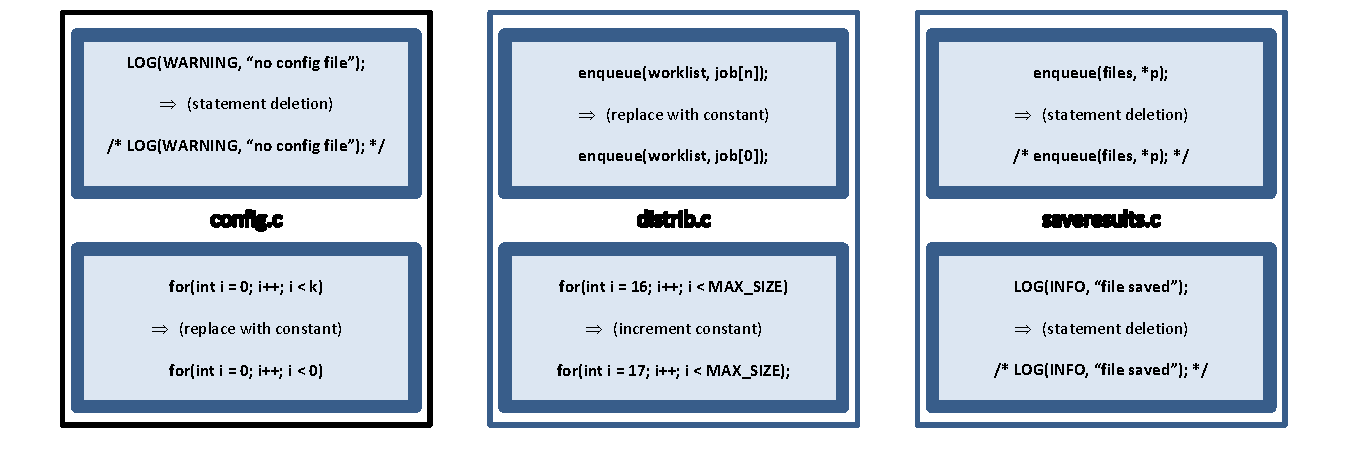
\includegraphics[width=0.95\columnwidth]{distmetric}

\caption{Which mutants are most similar?  If the user marked the
  mutant in the upper left corner as uninteresting and added a test
  to kill the
  mutant in the upper middle, which mutant
  should she examine next?}
\label{fig:distances}
\end{figure}


FPF requires a distance metric, and a distance metric requires a
\emph{representation} of mutants.  Mutants can be similar because they
modify the same line, function, class, or module, but also because,
despite being located in very different parts of a program, they are
very semantically similar.  E.g., a mutant to the parser of a compiler, to
an I/O error-handling routine in the code generator, and to a complex
optimization pass may all be very ``similar'' in the only meaningful
sense if all three mutants modify logging statements that don't have
any actual effect on the state of the compiler.  Figure
\ref{fig:distances} shows the fundamental problem.  It is not,
a priori, obvious which mutants here are most (dis-)similar.  Every
mutant has multiple plausible ``nearest neighbors'' --- another mutant
in the same file (likely to impact the same aspects of correctness),
another mutant with very similar code (likely to have the same kind of
semantic impact on the local context), or another mutant with the same operator (perhaps
likely to have some similarity, though probably of a lower importance
than the previous two types of similarity).  Are all logging statements
equivalent, or are only {\tt INFO} logging calls similar, while every
{\tt WARNING}, {\tt ERROR} or {\tt FATAL} is unique?  Some of these
decisions are likely to be project-independent, or even
developer-expertise-driven, and so a good metric
may well change during feedback-driven mutation testing, in response
to information from users (see Section \ref{sec:feedbackplan} below).

Elements of the
distance metric obviously include, at minimum, mutant location, mutation operator, and
some representation of the code element modified --- language
construct, functions called, variables modified, and so forth.  These
static aspects may also be augmented with user feedback (as noted
above), but also with dynamic information obtained during the process,
such as frequency with which tests cover the mutated
statements/modules, or the way the mutant changes the
program path from the unmutated code in tests.  PI Le Goues, with collaborators,
has proposed dynamic metrics over execution behavior for heuristic program repair,
including those measured over program state~\cite{desouza-gecco18,oliveira-ese18} and
observations of intermediate predicate behavior~\cite{Ding2019} (mutation testing
has strong conceptual analogies to program repair~\cite{Weimer2013}, suggesting
natural application of these prior measures to this new domain).

 In fact, there may
need to be two distance metrics:  one for selecting likely candidate
mutants to execute, that uses only static information and user
feedback, and one that uses dynamic results from compiling and testing
mutants to refine the notion of similarity for likely-novel mutants.
This is therefore a quite complex problem in representation and weighting of elements of a
representation, especially for a language- and
project- agnostic metric, that is also open to tuning via feedback
analysis.  One approach to the problem is to exploit metric learning
methods~\cite{kulis2012metric}, which were used in some of PI Groce's
previous work~\cite{SoftMining}.  But, to avoid over-fitting
to even a set of good examples, the final metric may have to be largely
hand-tuned, and designed to incorporate feedback and dynamically
extracted information, which is not easily handled with learned metrics.  In part this is due to the difficulty of establishing
large amounts of ground truth data, and the reality that
cross-project data will be less valuable than project-specific data
from users; there are unsupervised
approaches to metric
learning~\cite{scholkopf1998nonlinear,tipping1999probabilistic}, but most
popular approaches require supervision.

\subsection{Mutant Utility Predictor}

Novelty with respect to previously analyzed mutants is not the only
important characteristic of a mutant.  Presenting a novel, but likely
equivalent mutant is often a waste of time, though some equivalent
mutants can be useful for identifying optimization opportunities or
refactorings.  Furthermore, of two similar mutants next to be presented,
it is better to present one that is higher in the mutant dominance
hierarchy (the one such that its tests will kill more other mutants).
There has been some initial work on predicting mutant quality
attributes and utility~\cite{MutQuality,FaRM}, including estimating how hard mutants
will be to kill, statically.  In addition to advancing the
state-of-the-art in that respect, feedback-driven mutation testing
also requires determining how to balance the need for novelty and the
predicted utility of a mutant.  For example, a utility-driven ranking
might suggest avoiding a highly novel mutant because it is likely
equivalent; however, it may be that labeling this mutant as equivalent
lets the FPF ranking avoid numerous other similar mutants --- e.g.,
postponing labeling a logging statement as confirmed equivalent by the
user may be a bad idea.
%Also, if the mutant is \emph{not} equivalent (perhaps \emph{this} kind of logging needs to be tested), then the
%information is high-value.

\subsection{Feedback Analysis}
\label{sec:feedbackplan}

The ``feedback-driven'' aspect of feedback-driven mutation analysis
requires that information from the user be given high priority in the
process, a process with no clear equivalent in any previously proposed
mutation testing work.  The most straightforward example is that if a
user adds a test to kill a mutant, and marks that as a ``high impact''
action (the omitted testing was potentially allowing serious faults to
pass without detection) or even ``fault-revealing'' (the new test
detected a real fault in the system), then it may be most effective to
abandon the search for novelty and instead search for very similar
mutants still not killed by any test, in the expectation that these
may also result in high impact or fault-revealing tests.  If a user
marks a mutant as ``equivalent, but indicative of a refactoring
opportunity'', the same logic may apply:  similar mutants in other
parts of the code base may show the same problem with code quality,
even if they are predicted to be equivalent, and are not highly
novel.  In addition to informing the system of how useful various
analyzed mutants were, a user should also be able to inform the system
about correct and incorrect novelty rankings:  if the system presents
a mutant that is, from the user's POV, a (near-)duplicate of an
already handled mutant, the user should be able to express this fact,
and avoid future similar bad novelty estimates.

While large-scale crowdsourcing of user feedback is likely only
possible in some unusual industrial
settings~\cite{MutGoogle,ivankovic2018industrial}, it may also be
possible to apply mini-crowdsourcing techniques developed in the
context of testing machine-learning classifiers to mutant ranking and
analysis~\cite{Minicrowd}.  For high-visibility, high-criticality code
such as, e.g., Linux kernel modules, this may be a very powerful
tool.  The challenge in such a case is to allow communication between
feedback-driven mutation efforts, splitting work both so as to
minimize duplication and to target appropriate developers, as in automated assignment of
bug reports~\cite{bhattacharya2012automated,jonsson2016automated}.


\subsection{Mutation-Driven Development}

The primary focus of this project is to develop feedback-driven mutation
testing.  However, the ideas of Test-Driven Development
(TDD)~\cite{TDD,TDDFuture}, which repeatedly turns requirements into specific
test cases, then implements just enough functionality to pass the current tests,
can be generalized into a mutation-driven form.  A weakness of TDD is that the code will be narrowly tailored to the
requirements, which produce tests most effectively for ``shall''
type behaviors~\cite{INCOSE}.  But for security and
safety, ``shall not'' requirements that are omitted can be disastrous.
Mutation-Driven Development (MDD) in its simplest form would require an
application of feedback-driven mutation to the test suite at each development
step, to ensure that code not only does what the tests require, but that the
tests also sufficiently constrain the code to capture implicit shall-nots.
Since such a process implemented by modifying TDD-driven tests would likely
break the clean and appealing mapping between tests and requirements, and manual
tests are inherently weak, for high-criticality systems, MDD should focus on
augmenting TDD-driven tests with falsification-driven formal verification and
automated testing.  One way to do this would be to ``elaborate'' TDD-produced
unit tests into parameterized unit tests~\cite{UnitMeister,ParamUnit}, perhaps
using a tool like DeepState~\cite{DeepState} for C/C++.  In such a process,
weakness exposed by feedback-driven mutation testing would be addressed by
taking an existing unit test and generalizing some parameters and assertions to
kill the relevant mutants, letting, e.g., afl~\cite{aflfuzz},
libFuzzer~\cite{libfuzzer}, or a symbolic execution
tool~\cite{angr1,angr2,manticore} identify specific inputs.  The focus of the
MDD process would be on producing test harnesses~\cite{WODACommon,tstlsttt} that
can kill \emph{all} interesting mutants.  This aspect of the proposal
is better understood in terms of a scenario than as an explicit
research program:

\section{A Day in the Life of a Systems Programmer}

Laura is developing a data-management system for a NASA rover's software to be used during operation on another planet.  She is responsible both for a catalog process that handles data products, including critical configuration files, for other modules and the implementation of the low-level interface to custom, radiation-hardened, flash software.  Hardware changes have made certain design alterations to existing NASA-developed file systems essential, and Laura's expertise in the file system's performance has resulted in her also being assigned the task of constructing the higher-level module that gives access to the low-level persistent storage interface.

Laura has, in the process of developing the code, also developed a set of manually constructed unit tests and harnesses supporting automated test generation for the system.  She employs static analysis tools, with additional custom rules developed by the rover software team and the NASA facility's software tooling experts.  Laura has also added a few custom rules of her own that capture patterns she wants to enforce on herself with respect to the use of the low-level file system API.

Today, Laura is continuing an ongoing effort at changing functionality to the catalog and the file system, rewriting the ``rename'' call to provide a more restrictive set of allowed renames than the POSIX standard.  After reviewing the risks of arbitrary rename, the software team has agreed this is a restriction that protects the integrity of data better, while retaining all functionality ground operators might need to fix problems in the file system structure.  As part of this revision, Laura realized that without certain renames being allowed, a simpler scheme for enforcing atomicity of renames would work that could make mounting and checking the file system much easier.

Laura reaches a point where she believes her change is fully implemented and the tests have been revised to check the changed behavior.  She looks at a panel in her IDE showing Test Effectiveness, and notices that there are four Missed Bugs for her to examine.  She clicks on the top one, and the IDE focuses on a line of code in the rename function.  The display shows a change to that line, and says that altering the line in the way shown changes the file system binary but is not detected by any existing manual test or static analysis rule, and has not been detected in two minutes of fuzzing, across multiple cores, or by any stored fuzzing-generated test.

Laura thinks for a while about the change made, which involves passing a flag to the call that disables an expensive ``sanity check'' on header values for a file, to be used in contexts where the header has just been written and checked.  She thinks the current context is unsafe, and the check is required.  She knows that the danger is when there is a hardware failure of a certain kind, so she goes to the hardware emulator code that she uses to run tests without access to the rover testbeds, and requests the system to generate tests that target not just the mutated line of code (the system has already generated a number of these for her to examine), but the additional line with the relevant simulated hardware failure injection.  The fuzzers run in a targeted mode for a few minutes, and show Laura traces.  She runs some of these through a debugger, goes to the blackboard and calls in a colleague to discuss her reasoning.  They agree the check is indeed not needed, which will result in a small optimization in the file system.  Given the process she uses for developing her code, and the high quality of automated tests associated, Laura feels confident, given the argument, in optimizing the code.  The system now informs here that a very different mutant has the highest priority among uncaught bugs.  Of course, the system couldn't detect the mutant to the new version of the code, the one enabling the check, but Laura long ago informed the system that adding the check was never going to break any tests (the test is too cheap to produce interesting performance test violations, in any one location).  It therefore won't trouble her with this problem, now.  A small symbol attached to the parameter on the line of code does allow Laura to see that this line has an ignored unkilled mutant, which she can inspect if she is worried about the code.

Because Laura has been using the "MDD" process all along, her additional confidence tests will detect any problems with the optimization is not just based on mutation analysis of her current code.  Instead, it is based on mutants of all the versions of the design and functionaity she has implemented; if a problem is representable by a mutant of code no longer present (the older rename behavior, for example), then while not forming a basis for mutant alerts now, that behavior, in terms of API calls and hardware simulation choices, will be permanently in place in the stored corpus of fuzzing tests or manually constructed tests to address mutants.  So long as Laura allows the tool to guide her to always keep a high mutation score, she will keep these "mutant-regression" tests in place as an abstract form of the varying possibilities of her design, and the assurance tasks associated with that design perimeter.


\subsection{Core Research Questions}

The component-focused sections above provide an overview of the
research problems to be addressed by this proposal, but it is also
useful to consider the high-level research questions as a whole:

%\subsubsection{Feedback-Driven Mutation Testing
%Research Questions}

%\begin{framed}
\begin{enumerate}[labelsep=3pt,leftmargin=12pt]
\item What advances are required in order to maximize the efficiency
  and usability of any-language mutation?
\item How can a domain-specific language
enable new, more expressive mutation operators for
structural code changes
% that typically require a full fidelity parse
without compromising on the usability of a % simpler regex-based
regular
search-and-replace approach?
%\item How should the language of regular expressions be extended to allow
%  for language-agnostic definition of mutation operators that require
%  more parser-like analysis of code structure, without compromising
%  the usability and simplicity of the approach?
\item What is a good generalized, language-agnostic mutant representation
  and distance metric?
\item How can FPF-based selection of mutants for novelty best incorporate
  predictions of mutant equivalence, outcome, dominance, and
  productivity?  Is novelty or expected utility more important?
\item How can feedback-driven mutation testing most effectively
  incorporate feedback, including from crowds?
%\item Can mini-crowds be effectively leveraged to enhance the utility of user feedback?
%\item Is it possible to identify outliers in otherwise similar groups of
%  mutants?
\item How can we perform on-the-fly and parallel mutant evaluation/generation guided by
  (predicted) FPF?
\item Can we predict the \emph{cause} of mutant
  unkillability (e.g., oracle, coverage, equivalence, or nondeterminism)?
\item How can  we most effectively use already generated killing tests
  and counterexamples to prune mutants?
\item Is distance-based clustering plus timing information useful for quickly
  eliminating killable mutants similar to already-killed mutants?  How
  does this relate to Predictive Mutation Testing (PMT)?
  \item How can we integrate all of these aspects into a complete
    automated testing approach, and assist users in killing surfaced mutants?

\end{enumerate}
%\end{framed}

%\subsubsection{Any-Language Mutation Research Questions}

%\begin{framed}
% \begin{enumerate}[labelsep=3pt,leftmargin=12pt]
% \item What advances are required in order to maximize the efficiency and usability of a
%   fundamentally language-agnostic approach to
%   mutant generation?
% \item How can a domain-specific language
% enable new, more expressive mutation operators for
% structural code changes
% % that typically require a full fidelity parse
% without compromising on the usability of a % simpler regex-based
% regular
% search-and-replace approach?
% %\item How should the language of regular expressions be extended to allow
% %  for language-agnostic definition of mutation operators that require
% %  more parser-like analysis of code structure, without compromising
% %  the usability and simplicity of the approach?
% \item Is it possible to perform on-the-fly mutant generation for very
%   large projects, and reconcile this approach with FPF (e.g., generate
%   new mutants based on \emph{predicted} distances from
%   already evaluated mutants)?
% \end{enumerate}
%\end{framed}
